% titles: Quantum Choices

%% TO DO: what does a single particle quantum world without observers
%% look like?

%% naive realism about operators

%% what parts of the formalism correspond to natural-language talk of
%% properties?
%%
%% wave function realism

%% to do

%% TO DO: unitary dynamics -- linearity -- Wigner's theorem? 

%
% TO DO: Bloch sphere

% TO DO: dispersion (classical first)

% TO DO: uncertainty relation for spin ... see paper by Werner/

% contextual hidden variables

% determinism & deterministic theories (dynamics)

%% TO DO: transition probability

%% TO DO: Fourier transform for finite observables -- pictures 



\documentclass[12pt,fleqn]{article}
\usepackage{amsfonts,amssymb,amsthm,amsmath}
\title{Math for Quantum}
\author{Hans Halvorson}
\usepackage{tikz}
\usepackage{bm}

\renewcommand{\emph}{\textbf}

% \newcommand{\b}[1]{\mathbf{#1}}


\newcommand{\Ex}{\mc{E}}


\date{}

\newtheorem{thm}{Theorem}
\newtheorem{prop}{Proposition}
\theoremstyle{definition}
\newtheorem*{fact}{Fact}
\newtheorem*{defn}{Definition}
\newtheorem*{example}{Example}
\newtheorem{exercise}{Exercise}

\begin{document}

% \setcounter{chapter}{-1}

% \chapter{A primer on complex numbers}

\maketitle

\section{The complex numbers}

By definition, we let $i^2 = -1$, and we define $\mathbb{C}$ to be all
numbers of the form $a + ib$, where $a, b \in \mathbb{R}$.  The number
$a$ is called the \emph{real part} of $a+ib$, and the number $b$ is
called the \emph{imaginary part} of $b$.  That is,
$\mathrm{Re}(a+ib)=a$ and $\mathrm{Im}(a+ib)=b$.  We then define
addition and multiplication on $\mathbb{C}$ by
\[ \begin{array}{rcl}
    (a + ib) + (c + id) & = & (a + c) + i(b + d) ,\\
    (a + ib) \cdot (c + id) & = & (ac - bd) + i(bc + ad) .
  \end{array} \]
We define \emph{complex conjugation} by
\[ \begin{array}{rcl} \overline{a + bi} &= & a - bi . \end{array} \]
Note that $\frac{1}{2}(z+\overline{z})=\mathrm{Re}(z)$ and
$\frac{1}{2}(z-\overline{z})=\mathrm{Im}(z)$.

\begin{fact} Addition and multiplication on $\mathbb{C}$ are
  commutative and associative, and multiplication distributes over
  addition.  Every nonzero complex number $z$ has a unique
  multiplicative inverse, i.e.\ a complex number $z^{-1}$ such that
  $zz^{-1}=z^{-1}z=1$. \end{fact}


\begin{exercise} Show that $\overline{\overline{z}}=z$, and
  $\overline{z_1+z_2} =\overline{z_1} + \overline{z_2}$, and
  $\overline{z_1\cdot z_2}=\overline{z_1}\cdot
  \overline{z_2}$. \end{exercise}

For a complex number $z$, we say that $z\in\mathbb{R}$ when the
imaginary part of $z$ is zero.

\begin{exercise} Show that $\overline{z} = z$ iff $z\in \mathbb{R}$,
  and $\overline{z} = -z$ iff $z=ib$ for some $b \in
  \mathbb{R}$. \end{exercise}

\begin{exercise} Show that $\overline{z} z = a^2 +b^2$ when
  $z=a+ib$. \end{exercise}

\begin{defn} We define the \emph{modulus} of a complex number by
  $|z| =\sqrt{z\overline{z}}$. \end{defn}

\begin{exercise} Show that $|z_1\cdot z_2|=|z_2|\cdot |z_2|$.  Show
  that $|z|=0$ iff $z=0$.  \end{exercise}

For any complex number $z = a + bi$, if we define
$\theta = \tan (\frac{b}{a})^{-1}$, then
\[ z = |z| \left( \cos \theta + i\sin \theta \right) . \] This is
referred to as the \emph{polar representation} of $z$, and $\theta$ is
called the \emph{phase} of $z$.  Defining $r=|z|$ and
$e^{i\theta}=\cos \theta + i\sin \theta$, we can write
$z = r e^{i\theta}$.   In polar form, multiplication of complex
numbers has the following convenient representation:
\[
  (r_1 e^{i\theta _1})\cdot (r_2 e^{i\theta _2}) \: = \: (r_1r_2) e^{i
    (\theta _1+ \theta _2)} .\]

It is often convenient to represent the complex numbers on a plane,
with the real numbers as the horizontal axis and the imaginary numbers
as the vertical axis.  In this case, the modulus $r$ of
$re^{i\theta }$ corresponds to its distance from the origin, and the
phase $\theta$ corresponds to the angle that $re^{i\theta }$ makes
with the real axis.  What's more, we have
$\overline{re^{i\theta }}=re^{i(-\theta )}$, so that complex conjugation
corresponds to reflection in the real axis.

\begin{figure}[h!]
\centering
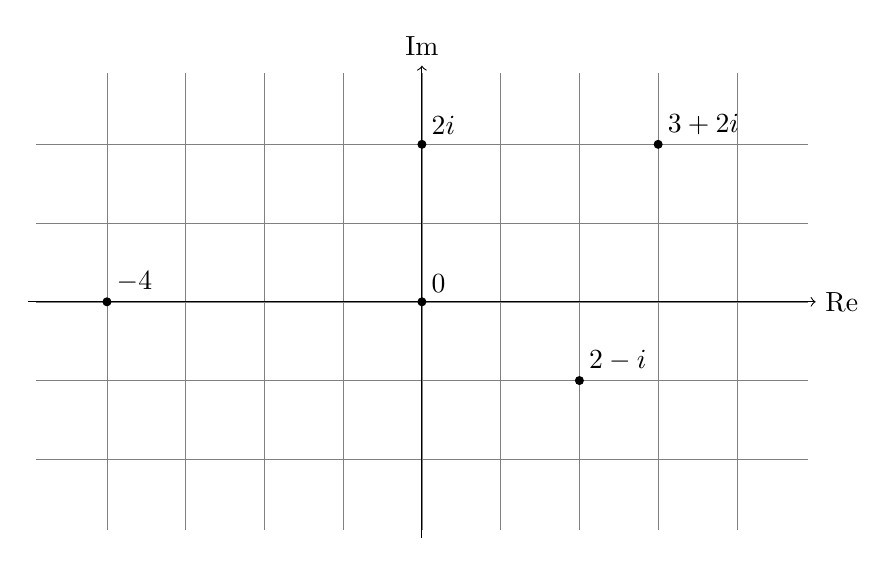
\begin{tikzpicture}
\draw[step=1cm,gray,very thin] (-4.9,-2.9) grid (4.9,2.9);
\draw[->] (-5,0) -- (5,0);
\draw[->] (0,-3) -- (0,3);
\node[above right] at (0,0) {$0$};
\node[above right] at (0,2) {$2i$};
\node[above right] at (3,2) {$3 + 2i$};
\node[above right] at (-4,0) {$-4$};
\node[above right] at (2,-1) {$2 -i$};
\node[shape=circle,inner sep=1pt,draw,fill=black] at (0,0) {};
\node[shape=circle,inner sep=1pt,draw,fill=black] at (0,2) {};
\node[shape=circle,inner sep=1pt,draw,fill=black] at (3,2) {};
\node[shape=circle,inner sep=1pt,draw,fill=black] at (-4,0) {};
\node[shape=circle,inner sep=1pt,draw,fill=black] at (2,-1) {};
\node[right] at (5,0) {$\mathrm{Re}$};
\node[above] at (0,3) {$\mathrm{Im}$};
\end{tikzpicture}
\end{figure}

\begin{figure}[h!]
\centering
\begin{tikzpicture}
\draw[->] (-0.1,0) -- (5,0);
\draw[->] (0,-0.1) -- (0,2.5);
\node[shape=circle,inner sep=1pt,draw,fill=black] at (3,2) {};
\node[right] at (3,2) {$z$};
\node[above left] at (1.5,1) {$r$};
\node[above] at (0.8,0) {$\theta$};
\draw[->] (0,0) -- (3,2);
\draw (5mm,0) arc (0:33:5mm);
\node[right] at (5,0) {$\mathrm{Re}$};
\node[left] at (0,2.5) {$\mathrm{Im}$};
\end{tikzpicture}
\end{figure}

\begin{defn} Let $\mathbb{T}=\{ z\in\mathbb{C}\mid |z|=1 \}$.  We say
  that $\mathbb{T}$ is the \emph{complex unit circle}. \end{defn}

Each unit-length complex number is of the form
$e^{i\theta }=\cos \theta +i\sin \theta$, and multiplication on
$\mathbb{T}$ can be represented as
$e^{i\theta _1}e^{i\theta _2}=e^{i(\theta _1+\theta _2)}$.  Hence
$(e^{i\theta })^{-1}=e^{-i\theta }$.  We also have the famous
\emph{Euler identity}:
\[ e^{i\pi } \: = \: \cos \pi + i\sin \pi \: = \: -1 .\]

\section{Vector spaces}

A \emph{complex vector space} is a set $V$, equipped with
	\begin{itemize}
	\item
	a special \emph{zero} element $\mathbf{0}$,
	\item
	an \emph{addition} operation $+: V \times V \to V$, and
	\item
	a \emph{scalar multiplication} operation $\cdot : \mathbb{C} \times V \to V$,
	\end{itemize}
such that for any $u, v, w \in V$ and $\alpha, \beta \in \mathbb{C}$,
\[ \begin{array}{rcl}
u + v &= & v + u\\
u + (v + w) &= & (u + v) + w\\
v + \mathbf{0} &= &  v \\
0\cdot v &= &  \mathbf{0}\\
1 \cdot v &= &  v\\
\alpha \cdot (\beta \cdot v) &= & (\alpha\beta) \cdot v\\
\alpha\cdot(u + v) &= & \alpha \cdot u + \alpha \cdot v\\
(\alpha + \beta) \cdot v &= & \alpha \cdot v + \beta \cdot v
\end{array} \]
We will henceforth abbreviate scalar multiplication $\alpha \cdot v$
by $\alpha v$.

\begin{exercise} Show that $v+(-1)v=\mathbf{0}$. \end{exercise}

\begin{defn} A \emph{basis} for $V$ is a collection of vectors
  $v_i \in V$ such that any $v \in V$ can be expressed uniquely in the
  form $v = \sum_i \alpha_i v_i$.  The \emph{dimension} of vector
  space $V$ is the smallest number $n$ such that there exists a basis
  consisting of $n$ vectors.  We write $\dim V=n$.  \end{defn}

\begin{example} 


\end{example}

\begin{defn} 
  A \emph{subspace} of a vector space $V$ is a nonempty subset
  $W\subseteq V$ that is closed under addition and scalar
  multiplication.  In other words, $W$ is itself a vector space inside
  of $V$ such that $\dim W\leq \dim V$.  In the finite-dimensional
  case, $\dim W=\dim V$ only if $W=V$.  \end{defn}

\begin{defn} Given a complex vector space $V$, an \emph{inner product}
  is a binary operation
  $\langle - ,-\rangle :V \times V \to \mathbb{C}$ such that for any
  $u, v, w \in V$ and $c\in \mathbb{C}$,
\[ \begin{array}{rcl}
\langle u, v\rangle &= & \overline{\langle v, u\rangle}\\
\langle u,v + w\rangle &= &  \langle u, v\rangle + \langle u, w\rangle
\\
\langle u,cv\rangle & = & c\langle u,v\rangle \\
\langle u, u\rangle & \geq & 0 \end{array} \] The  \emph{norm} of a vector $v$
is defined to be $\| v\| = \sqrt{\langle v, v\rangle}$.  \end{defn}

\begin{prop}[Cauchy-Schwartz inequality]
  $|\langle u,v\rangle |\leq \langle u,u\rangle \cdot \langle
  v,v\rangle$. \end{prop}

\begin{defn} Two vectors $u, v \in V$ are said to be \emph{orthogonal}
  if $\langle u, v\rangle = 0$. \end{defn}

\begin{defn} An \emph{orthonormal} basis for $V$ is a basis consisting
  entirely of vectors of norm 1, which are all orthogonal to one
  another. \end{defn}

\begin{defn} A \emph{finite-dimensional Hilbert space} is a
  finite-dimensional complex vector space equipped with an inner
  product. \end{defn}

We use elements of a Hilbert space $H$ to represent the so-called
``pure'' states of a quantum system.  Unlike in the classical case,
one cannot determine whether or not the system is in the state
represented by $v$ through a single measurement.  The best one can do
is find a measurement setup such that for any state $v$, the
probability of a positive result is given by
\begin{equation}
  \frac{|\langle v, w\rangle|^2}{\| v\| ^2 \| w\| ^2}
\end{equation}
Hence, for any $\alpha \in \mathbb{C}$ and $\psi \in H$, the states
represented by $\psi$ and $\alpha \psi$ cannot be discriminated from
one another; we therefore take them to be the same state.  We use this
freedom to stipulate that only the \emph{unit norm} elements of a
Hilbert space (those such that $\| v\| = 1$) will be used to represent
states.  Under this stipulation, the probability of a positive result
in the ``$\psi$-test'' is then simply given by
$|\langle\phi, \psi\rangle |^2$.  Note that even with this
stipulation, there are still multiple elements of $H$ representing the
same state: e.g., $v$ and $iv$.

\begin{example} Consider the two-dimensional vector space $V$.  We can
  represent elements of $V$ by ordered pairs (or by column vectors),
  and we can define an inner product on $V$ by
  \[ \langle (a,b) ,(c,d) \rangle = \: a^*c+b^*d .\] In this case, the
  pair $(1,0)$ and $(0,1)$ form an orthonormal basis for $V$.
\end{example}



\section{Linear operators}

\begin{defn} Let $V$ and $W$ be a vector spaces over $\mathbb{C}$, and
  let $A:V\to W$ be a function.  We say that $A$ is \emph{linear} just
  in case $A(v+w)=Av+Aw$ and $A(cv)=cAv$, for all $v,w\in V$ and all
  $c\in\mathbb{C}$.  For the case where $A:V\to V$, we say that $A$ is
  a \emph{linear operator}.  \end{defn}

You may well have seen linear operators before, but most likely under
the name \emph{matrices}.  That's because matrices provide a
particularly convenient way for representing linear operators on
finite-dimensional vector spaces.  Here an $n\times n$ matrix (over
$\mathbb{C}$) is an array of $n^2$ complex numbers.  For the most
part, it will suffice for us to look at the simplest non-trivial case,
i.e.\ $2\times 2$ matrices.  Let $A$ be the matrix
\[ \begin{pmatrix} a_{11} & a_{12} \\ a_{21} & a_{22} \end{pmatrix} . \] Then the
  action of $A$ on a vector $\begin{pmatrix} b_1 \\ b_2 \end{pmatrix}$
  can be computed as follows:
  \[ \begin{pmatrix} a_{11} & a_{12} \\ a_{21} &
      a_{22} \end{pmatrix} \begin{pmatrix} b_1 \\ b _2 \end{pmatrix}
    \: = \: \begin{pmatrix} a_{11}b_1 + a_{12}b_2 \\ a_{21}b_1 +
      a_{22}b_2 \end{pmatrix} . \] We've already defined a product of
  linear operators in terms of composition.  You can then verify (by a
  straightforward calculation) that this product yields the standard
  matrix multiplication rule:
  \[ \begin{pmatrix} a_{11} & a_{12} \\ a_{21} &
      a_{22} \end{pmatrix} \begin{pmatrix} b_{11} & b_{12} \\ b _{21}
      & b_{22} \end{pmatrix}
    \: = \: \begin{pmatrix} a_{11}b_{11}+a_{12}b_{21} & a_{11}b_{12}+a_{12}b_{22} \\ a_{21}b_{11} +
      a_{22}b_{21} & a_{21}b_{12}+a_{22}b_{22} \end{pmatrix} . \]

\begin{defn} A \emph{linear functional} on $V$ is a linear map from
  $V$ to $\mathbb{C}$. \end{defn}

Interestingly, the linear functionals on a vector space $V$ themselves
form another vector space $V^*$.  In particular, given linear
functionals $\rho$ and $\sigma$, define $\rho +\sigma$ pointwise,
i.e.\ $(\rho +\sigma )(v)=\rho (v)+\sigma (v)$.  Similarly, given a
complex number $c$, define $(c\rho )(v)=c\rho (v)$.  We call $V^*$ the
\emph{dual space} of $V$.

\begin{thm}[Riesz representation] Let $V$ be a finite-dimensional
  vector space, and let $\rho :V\to \mathbb{C}$ be a linear
  functional.  Then there is a unique vector $w\in V$ such that
  $\rho (v)=\langle w,v\rangle$, for all $v\in W$. \end{thm}


\begin{prop} Let $V$ be a finite-dimensonal vector space.  If
  $A:V\to W$ is linear, then there is a unique linear operator
  $A^*:W\to V$ such that $\langle w,Av\rangle =\langle A^*w,v\rangle$,
  for all $v\in V$ and $w\in W$. \end{prop}

\begin{fact} In a matrix representation of linear operators, the
  matrix for the operator $A^*$ is the conjugate transpose of the
  matrix for the operator $A$. \end{fact}

\begin{defn} Let $A$ be a linear operator.  Then we define:
  \begin{itemize}
   \item $A$ is \emph{normal} if $A^*A=AA^*$. 
   \item $A$ is \emph{self-adoint} if $A^*=A$.
   \item $A$ is \emph{unitary} if $A^*A=AA^*=I$. \end{itemize} \end{defn}

\begin{example}[spin operators] Consider the two-dimensional vector space $V$, whose
  elements we will represent by column vectors.  We define the
  function $\sigma _x:V\to V$ to take $(a,b)$ to
  $\frac{1}{2}(a,-b)$. Clearly $\sigma _x$ is linear.  In fact,
  $\sigma _x$ can be represented as the matrix
  \[ \sigma _x \: = \: \frac{1}{2}\begin{pmatrix} 1 & 0 \\ 0 &
      -1 \end{pmatrix} .\] It's easy to see then that
  $\sigma _x^*=\sigma _x$, and $\sigma _x\sigma _x=1$.  Hence,
  $\sigma _x$ is both self-adjoint and unitary.  \end{example}


\section{Composite systems}


%% TO DO: dynamics





\end{document}
%%% Local Variables:
%%% mode: latex
%%% TeX-master: t
%%% End:
